\subsection{Multinational Operations}

\begin{remark} \hlt{Foreign Currency on MNC}
\begin{enumerate}[label=\roman*.]
\setlength{\itemsep}{0pt}
\item MNC may engage in business transactions denominated in foreign currency
\item MNC may invest in subsidiaries that maintain their books and records in foreign currency
\end{enumerate}
\end{remark}

\begin{definition} Currency Types
\begin{enumerate}[label=\roman*.]
\setlength{\itemsep}{0pt}
\item \hlt{Local Currency}: currency where the company operates.
\item \hlt{Functional Currency}: currency of the primary economic environment in which the entity operates. The currency in which the entity generates and expends cash. May be in local currency or some other currency.
\item \hlt{Presentation Currency}: currency in which the parent company prepares its financial statements.
\end{enumerate}
\end{definition}

\begin{flushleft}
\begin{tabularx}{\textwidth}{p{8em}|X|p{11em}|p{11em}}
\hline
\rowcolor{gray!30}
Transaction & Type of Exposure & Foreign Curr Strengthen & Foreign Curr Weaken \\
\hline
Export sale & Asset (account receivable) & Gain & Loss \\
\hline
Import purchase & Liability (Account payable) & Loss & Gain \\
\hline
\end{tabularx}
\end{flushleft}

\begin{remark} \hlt{Exposure to Transaction Exposure} \\
Transaction exposure are related to imports and exports:
\begin{enumerate}[label=\roman*.]
\setlength{\itemsep}{0pt}
\item Import Purchase: importer pay in foreign currency and allowed to defer payment. Exposed to risk that foreign currency appreciate, increasing functional currency amount required to acquire foreign currency.
\item Export Sale: exporter paid in foreign currency and allowed payment to be deferred. Exposed to risk that foreign currency depreciate, decreasing functional currency which the foreign currency can be converted.
\end{enumerate}
\end{remark}

\begin{definition} \hlt{Foreign Currency Risk}\\
Risk arises only when transaction date and payment date are different.\\
If balance sheet date occurs before transaction is settled, foreign currency gain and loss are recognised on IS.\\
Subsequent gains and losses are recognised from BS date through the settlement date. Adding gain and losses for both accounting periods produces amount equal to actual realised gain or loss on foreign currency transaction.
\end{definition}

\begin{remark} \hlt{Disclosure of Transaction Gains and Losses}\\
IFRS, GAAP do not require disclosure of where such gains and losses would be recorded. Typically placed as:
\begin{enumerate}[label=\roman*.]
\setlength{\itemsep}{0pt}
\item a component of other operating income/expense; or
\item a component of non-operating income/expense; or
\item as part of net financing cost
\end{enumerate}
Operating profit margin is then affected by where the gain and loss is placed.
\end{remark}

\subsubsection{Translation of Foreign Currency Financial Statements}

\begin{method} Methods to remeasure or translate financial statements are as follows:
\begin{enumerate}[label=\roman*.]
\setlength{\itemsep}{0pt}
\item \hlt{Re-measurement}: converting local currency into functional currency using temporal method
\item \hlt{Translation}: converting functional currency into parent presentation currency with current rate method.
\end{enumerate}
The method chosen is determined by functional currency relative to parent presentation currency.
\end{method}

\begin{method} \hlt{IFRS on Deciding on Functional Currency}
\begin{enumerate}[label=\roman*.]
\setlength{\itemsep}{0pt}
\item Currency mainly influences sales prices for goods and services
\item Currency of country whose competitive forces and regulations mainly determine the sales price of its goods and services
\item Currency that mainly influences labour, material, and other costs of providing goods and services
\item Currency in which funds from financing activities are generated
\item Currency in which receipts from operating activities are usually retained.
\end{enumerate}
To determine in whether the foreign entity functional currency is same as parent functional currency:
\begin{enumerate}[label=\roman*.]
\setlength{\itemsep}{0pt}
\item If the activities of foreign operation are an extension of parent, or are autonomous
\item If transactions with parent is large or small proportion of foreign entity activities
\item If CF generated by foreign entity directly affect CF of parent and are available to be remitted to parent
\item If operating CF generating by foreign operations are sufficient to service existing and normally expected debt; or whether the foreign entity will need funds from the parent to service its debt
\end{enumerate}
\end{method}

\begin{method} \hlt{Determining Appropriate Translation Method}
\begin{enumerate}[label=\roman*.]
\setlength{\itemsep}{0pt}
\item Current Rate Method: $\text{Functional Currency} \neq \text{Presentation Currency}$.\\
Translation involves self-contained, independent subsidiaries whose operating, investing, and financing activities are decentralised from the parent.
\item Temporal Method: $\text{Functional Currency} = \text{Presentation Currency}$.\\
Re-measurement occurs when subsidiary is well integrated with the parent.
\item Monetary/Non-Monetary (Mixed) Method: $\text{Local Currency} \neq \text{Functional Currency} \neq \text{Presentation Currency}$.\\
Temporal method used to remeasure from local currency into functional currency, then current rate method used to translate functional currency into presentation currency.
\item Hyper-inflationary Environment:
\begin{enumerate}[label=\arabic*.]
\setlength{\itemsep}{0pt}
\item IFRS: subsidiary financial statements restated for inflation, translated using current exchange rate
\item GAAP: functional currency considered to be parent's presentation currency, temporal method used
\end{enumerate}
\end{enumerate}
\end{method}

\begin{figure}[H]
\centering
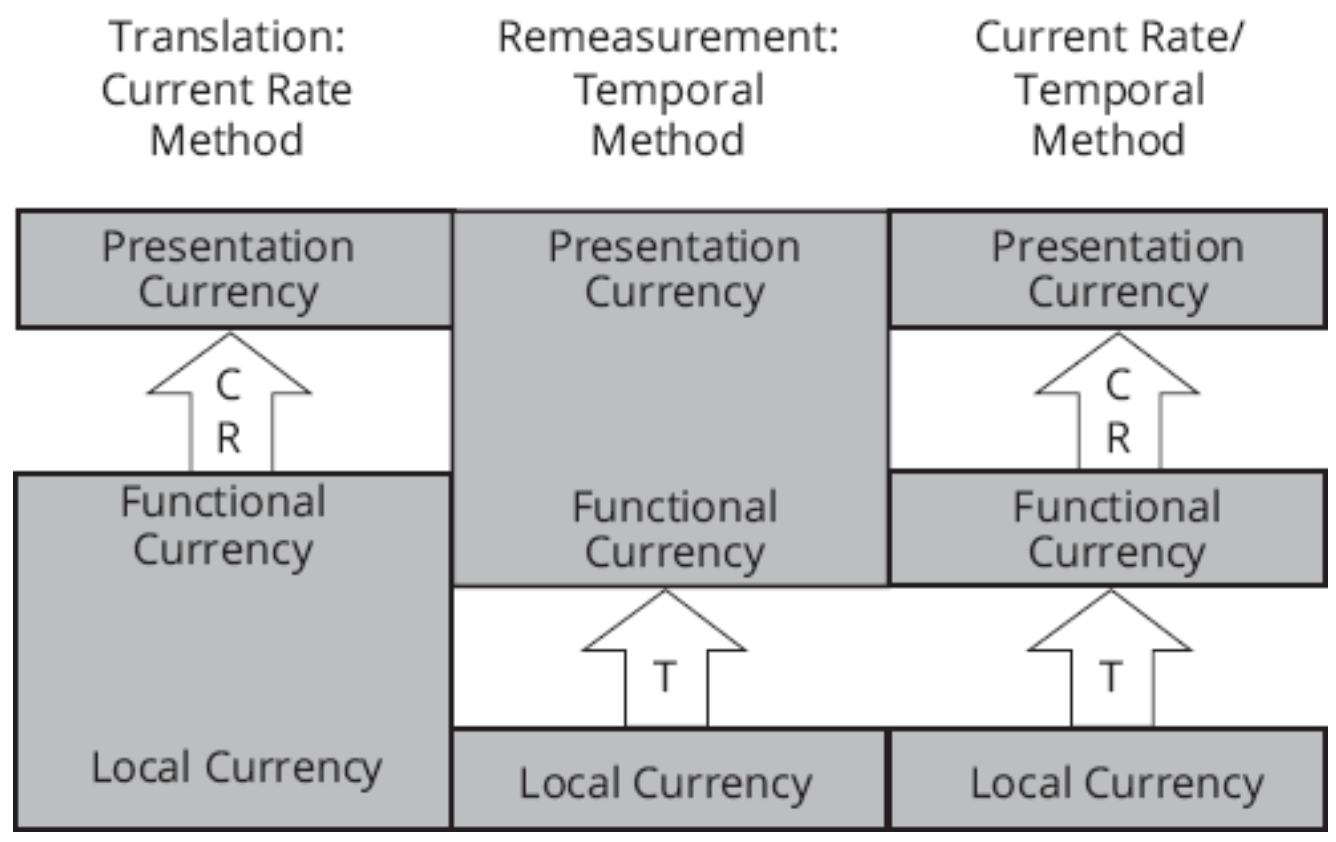
\includegraphics[scale=0.4]{fsa/translation}
\caption{Translation and re-measurement methods}
\end{figure}

\begin{definition}{\color{white}space}
\begin{enumerate}[label=\roman*.]
\setlength{\itemsep}{0pt}
\item \hlt{Current Rate}: exchange rate on balance sheet date
\item \hlt{Average Rate}: average exchange rate over reporting period
\item \hlt{Historical Rate}: actual rate in effect when original transaction occured
\end{enumerate}
\end{definition}

\begin{remark} \hlt{Temporal Method on Inventory and COGS}
\begin{enumerate}[label=\roman*.]
\setlength{\itemsep}{0pt}
\item FIFO: ending inventory remeasured based on more recent rates. However, COGS consists of costs that are older; hence exchange rates used to remeasure COGS are older.
\item LIFO: ending inventory remeasured based on older costs. However, COGS consists of costs from most recently purchased goods; hence COGS is remeasured based on more recent exchange rates.
\item Weighted-Average: ending inventory and COGS remeasured with weight-average exchange rate
\end{enumerate}
\end{remark}

\begin{remark} \hlt{Temporal Method Overview}\\
Translation adjustment needed to keep translated BS in balance is reported as gain or loss in net income (GAAP: re-measurement gains and losses).\\
Method results in either net asset or net liabilities (if exposed asset greater than or less than liabilities).
\end{remark}

\begin{remark} \hlt{Current Rate Method Overview}\\
Entire investment in foreign entity is exposed to translation gain or less. Hence all assets and liabilities must be revalued at each BS date. Net translation gain and loss is unrealised except when entity is sold; this is cumulated and deferred on BS as separate component of stockholder equity.\\
Method results in net asset BS exposure (as total assets greater than total liabilities).
\end{remark}


\begin{flushleft}
\begin{tabularx}{\textwidth}{p{25em}|X|X}
\hline
\rowcolor{gray!30}
Translation Item & Current Rate & Temporal \\
\hline
\bf{Assets} & & \\
Monetary (e.g., cash, receivables) & Current rate & Current rate \\
Non-monetary & & \\
\xxx measured at current value (marketable securities etc.) & Current rate & Current rate \\
\xxx measured at historical costs (PPE, intangibles etc.) & Current rate & Historical rate \\
\hline
\bf{Liabilities} & & \\
Monetary (accounts payable, accrued expenses, LT debt, deferred income taxes) & Current rate & Current rate \\
Non-monetary & & \\
\xxx measured at current value & Current rate & Current rate \\
\xxx Not measured at current value (e.g., deferred revenue) & Current rate & Historical rate \\
\hline
\bf{Equity} & & \\
Other than retained earnings & Historical rate & Historical rate \\
Retained earnings & Historical rat$\text{e}^1$ & Historical rat$\text{e}^1$ \\
\hline
\bf{Revenues and SG\&A} & Average rate & Average rate \\
\hline
\bf{Expenses} & & \\
Most expenses & Average rate & Average rate \\
Expenses related to assets translated at historical rates (i.e., COGS, depreciation, amortisation) & Average rate & Historical rate \\
Translation adjustment on parent financial statement & Equit$\text{y}^2$ & Net Income GnL \\
\hline
Common Stock & Historical rate & Historical rate \\
Cost of Goods Sold & Average rate & Historical rate \\
Depreciation and Amortisation & Average rate & Historical rate \\
Net Income & Average rate & Mixed rate \nonumber \\
Equity (as a whole) & Current rate & Mixed rate \\
Exposure & Net assets & Net monetary assets \\
\hline
\end{tabularx}
\end{flushleft}
\begin{enumerate}[label=\arabic*., before=\small]
\setlength{\itemsep}{0pt}
\item Beginning balance plus translated net income less dividends translated at historical rate
\item Accumulated as separate component of equity
\end{enumerate}

\begin{remark} \hlt{Translation Adjustments}
\begin{flushleft}
\begin{tabularx}{\textwidth}{p{10em}|X|X}
\hline
\rowcolor{gray!30}
BS Exposure & Local Currency Appreciates & Local Currency Depreciates \\
\hline
Net Assets & Positive & Negative \\
\hline
Net Liabilities & Negative & Positive \\
\hline
\end{tabularx}
Cumulative translation adjustment is used to keep translated BS in balance; this is sum of translation adjustments over successive accounting periods.
\end{flushleft}
\end{remark}

\begin{remark} \hlt{Exposure to Changing Exchange Rates}
\begin{enumerate}[label=\roman*.]
\setlength{\itemsep}{0pt}
\item Current Rate Method: exposure is the net asset position of subsidiary (if assets exceeds its liabilities).\\
If subsidiary has net asset exposure, and local currency is appreciating, a gain is recognised.\\
A net asset exposure in depreciating environment will result in a loss.\\
Firm with net liability position is unusual; most firm can't survive very long in this scenario.
\item Temporal method: Only monetary assets and liabilities exposed to changing rates.\\
If monetary liabilities exceed monetary assets, firm has net monetary liability exposure.
Net monetary liability exposure (NMLE) when foreign currency is appreciation results in a loss.\\
Net monetary liability exposure coupled with depreciating currency will result in a gain.\\
Firms may limit exposure by balancing monetary assets and monetary liabilities.
\end{enumerate}
\end{remark}

\begin{method} \hlt{Translation of Retained Earnings} \\
At end of first year, foreign currency (FC) retained earnings (R/E) are translated into parent currency (PC):
\begin{flushleft}
\begin{tabularx}{\textwidth}{Xp{20em}X}
\hline
Net income in FC & [Translated with method used to translate IS] & $=$ Net income in PC \\
$-$ Dividends in FC & $\times$ Exchange rates when dividends declared & $=$ $-$ Dividends in PC \\
\hline
R/E in FC & & R/E in PC
\end{tabularx}
\end{flushleft}
Retained earnings in PC at end of first year become beginning retained earnings in PC for second year. The retained earnings in second and subsequent years are calculated as follows:
\begin{flushleft}
\begin{tabularx}{\textwidth}{Xp{20em}X}
\hline
Beginning R/E in FC & [From last year's translation] & $\rightarrow$ Beginning R/E in PC \\
$+$ Net income in FC & [Translated with method used to translate IS] & $=$ $+$ Net income in PC \\
$-$ Dividends in FC & $\times$ Exchange rates when dividends declared & $=$ $-$ Dividends in PC \\
\hline
End R/E in FC & & End R/E in PC
\end{tabularx}
\end{flushleft}
\end{method}

\begin{remark} \hlt{Currency Exchange Rate Movement on Financial Statements}
\begin{flushleft}
\begin{tabularx}{\textwidth}{p{10em}|X|X|X}
\hline
\rowcolor{gray!30}
 & Temporal, NMLE & Temporal, NMAE & Current Rate \\
\hline
Foreign Appreciation &
\xxx $\uparrow$ Revenues
\xxx $\uparrow$ Assets 
\xxx $\uparrow$ Liabilities
\xxx $\downarrow$ Net Income
\xxx $\downarrow$ Shareholder's equity
\xxx Translation loss &
\xxx $\uparrow$ Revenues
\xxx $\uparrow$ Assets 
\xxx $\uparrow$ Liabilities
\xxx $\uparrow$ Net Income
\xxx $\uparrow$ Shareholder's equity
\xxx Translation gain &
\xxx $\uparrow$ Revenues
\xxx $\uparrow$ Assets 
\xxx $\uparrow$ Liabilities
\xxx $\uparrow$ Net Income
\xxx $\uparrow$ Shareholder's equity
\xxx $+$ Translation Adjust
\\
\hline
Foreign Depreciation & 
\xxx $\downarrow$ Revenues
\xxx $\downarrow$ Assets 
\xxx $\downarrow$ Liabilities
\xxx $\uparrow$ Net Income
\xxx $\uparrow$ Shareholder's equity
\xxx Translation loss &
\xxx $\downarrow$ Revenues
\xxx $\downarrow$ Assets 
\xxx $\downarrow$ Liabilities
\xxx $\downarrow$ Net Income
\xxx $\downarrow$ Shareholder's equity
\xxx Translation gain &
\xxx $\downarrow$ Revenues
\xxx $\downarrow$ Assets 
\xxx $\downarrow$ Liabilities
\xxx $\downarrow$ Net Income
\xxx $\downarrow$ Shareholder's equity
\xxx $-$ Translation Adjust\\
\hline
\end{tabularx}
\end{flushleft}
\end{remark}

\begin{remark} \hlt{Current Rate Method on Financial Ratios}\\
Let pure ratios be ratios consisting of components from a single financial statement, i.e., BS only, IS only.
\begin{enumerate}[label=\roman*.]
\setlength{\itemsep}{0pt}
\item Pure balance sheet and pure income statement ratios unaffected (local currency trends are preserved)
\item If foreign currency is depreciating (appreciating), translated mixed ratios (with IS item in numerator, end-of-period BS item in denominator) will be larger (smaller) than original ratio.
\end{enumerate}
\end{remark}

\begin{method} \hlt{Procedure for Analysis of Choice of Method on Ratio}
\begin{enumerate}[label=\roman*.]
\setlength{\itemsep}{0pt}
\item Determine whether the foreign currency is appreciating or depreciating
\item Determine the rate (historical, average, or current) used to convert the numerator under both methods. Determine if the numerator of the ratio will be same, larger, or smaller under both methods.
\item Determine the rate (historical, average, or current) used to convert the denominator under both methods. Determine if the denominator of the ratio will be same, larger, or smaller under both methods.
\item Determine whether the ratio will increase, decrease, or stay the same based on direction of change in numerator and denominator.
\end{enumerate}
\end{method}

\subsubsection{Hyper-Inflationary Economy}

\begin{definition} \hlt{Hyper-Inflationary Environment}\\
Economy where cumulative inflation is approaching or is over $100\%$ in three-year period.
\end{definition}

\begin{method} \hlt{Reporting in a Hyper-Inflationary Environment}
\begin{enumerate}[label=\roman*.]
\setlength{\itemsep}{0pt}
\item IFRS:
\begin{enumerate}[label=\arabic*.]
\setlength{\itemsep}{0pt}
\item BS monetary assets and monetary liabilities not restated
\item BS non-monetary assets and non-monetary liabilities restated for inflation using price index. As non-monetary items are carried at historical cost, multiply original cost by change in price index for the period between acquisition date and balance sheet date.
\item BS components of shareholder's equity (other than retained earnings) restated by applying change in price index from beginning of period or date of contribution if later
\item BS retained earnings will be residual figure that balances the balance sheet
\item IS items restated by multiplying change in price index from the date the transactions occur
\item IS net purchasing power gain or loss recognised based on the net monetary asset or liability exposure.\\
Holding monetary assets during inflation results in purchasing power loss.\\
Holding monetary liabilities during inflation results in purchasing power gain.\\
This forces net income to be same as net income that was residual in statement of retained earnings.
\end{enumerate}
Once subsidiary's financial statements are adjusted for inflation, these are translated into parent reporting currency using current exchange rate.
\item GAAP: Temporal method used. Require foreign entity financial statements to be remeasured as if functional currency were the reporting currency.
\end{enumerate}
\end{method}

\begin{remark} \hlt{Inflation Method vs Temporal Method}
\begin{enumerate}[label=\roman*.]
\setlength{\itemsep}{0pt}
\item Under temporal method, monetary assets and liabilities are exposed to changing exchange rates.\\
In inflation method, the monetary assets and liabilities are exposed to risk of inflation.
\item Purchasing power GnL analogous to exchange rate GnL when foreign currency is depreciating.
\item Re-measurement GnL is recognised in IS, as is net purchasing power GnL from inflation.
\end{enumerate}
\end{remark}

\subsubsection{Disclosures for Multinational Operations}

\begin{remark} \hlt{Disclosures on Translation Method}\\
IFRS and GAAP require two types of disclosures:
\begin{enumerate}[label=\roman*.]
\setlength{\itemsep}{0pt}
\item amount of exchange differences recognised in net income; and
\item amount of cumulative translation adjustment classified in a separate component of equity, along with reconciliation of amount of cumulative translation adjustment at the beginning and end of the period.
\end{enumerate}
GAAP specifically also requires disclosure of amount of translation adjustment transferred from stockholder equity and included in current income from disposal of foreign entity.\\
The amount of exchange differences recognised in net income consists of:
\begin{enumerate}[label=\roman*.]
\setlength{\itemsep}{0pt}
\item foreign currency translation gains and losses, and
\item translation gains and losses resulting from application of temporal method.
\end{enumerate}
\end{remark}

\begin{definition} {\color{white}space}
\begin{enumerate}[label=\roman*.]
\setlength{\itemsep}{0pt}
\item \hlt{Clean Surplus Accounting}: all non-owner changes in equity equity, such as translation adjustments are included in determination of net income.
\item \hlt{Dirty Surplus Accounting}: some income items are reported as part of shareholder's equity, rather than as gains and losses on income statement
\end{enumerate}
\end{definition}

\begin{definition} {\color{white}space}
\begin{enumerate}[label=\roman*.]
\setlength{\itemsep}{0pt}
\item \hlt{Effective tax rate}: tax expense divided by pretax profit, in income statement
\item \hlt{Statutory tax rate}: tax rate by the home country
\item \hlt{US Tax Regime}: MNC owes taxes on foreign income only to extent that the US corporate tax exceeds foreign rate of tax on that income. Foreign income earned by US MNC is not taxed until it is repatriated.
\end{enumerate}
\end{definition}

Entity with operations in multiple countries may aim to set transfer prices such that higher portion of its profit is allocated to lower tax jurisdictions.

\begin{remark} \hlt{Disclosures on Tax Implications}\\
Accounting standards require companies to provide reconciliation between effective and statutory tax rate. The reconciliation disclosure can be used to project future tax expense.
\end{remark}

\begin{remark} Changes in effective tax rate on account of foreign operations can be due to:
\begin{enumerate}[label=\roman*.]
\setlength{\itemsep}{0pt}
\item Changes in mix of profits from different countries with varying tax rates
\item Changes in the tax rates
\end{enumerate}
\end{remark}

\begin{remark} \hlt{Disclosures Related to Sales Growth}\\
Foreign currency effects on sales are disclosed in MD\&A section of annual reports.\\
Growth in sales due to changes in volume, price is more sustainable than those from changes in exchange rates.
\end{remark}

\begin{remark} \hlt{Disclosures Related to Major Sources of Foreign Exchange Risk}\\
Disclosures in MD\&A include sensitivity analysis, with information on major sources of foreign exchange risk given its country of operations, and disclosure of profit impact of a given change in exchange rates.
\end{remark}